\section{Debunk esercizi PIA}
In questo paragrafo verrà commentato il codice diffuso sul canale Teams e presentato a lezione relativo alle esercitazioni sulla PIA (Marzo 2025).

% \subsection{Esercizio 2}\label{par:es_1_2}
% Il programma serve a provare una semplice configurazione costituita da due sistemi S1 ed S2 dotati entrambi di un processore M68000, una ROM di 8K (addr \$0-\$1FFF), una RAM di 10K (addr \$8000-\$A7FF) e un device parallelo PIA mappato a \$2004. I due PIA sono interconnessi tra loro e mediante un protocollo di handshaking consentono ai due sistemi di scambiarsi un messaggio. In particolare, il sistema S1 trasferisce un vettore di N caratteri verso il sistema S2 sul porto parallelo. Il messaggio si trova in un'area di memoria del sistema S1 e viene salvato in una ulteriore area di memoria nel sistema S2. Questa volta, anche la trasmissione è gestite tramite interrupt e non tramite polling come nel paragrafo \ref{par:es_1_1}.

% \subsubsection{Sistema S1}
% Questo driver serve per la programmazione del sistema S1, che effettua il trasferimento sotto interrupt.
% Per quanto riguarda l'area dati valgono le stesse considerazioni fatte per l'esercizio 1 (\ref{par:es_1_1_1}), con l'aggiunta dell'allocazione di una variabile COUNT anche per il trasmettitore. 

% \begin{lstlisting}
%     ***AREA MAIN***
% 	ORG    $8200

% PIADB	EQU    $2006	;indirizzo di PIA-B dato, usato in output 
% PIACB	EQU    $2007	;indirizzo di PIA-B controllo

% MAIN	JSR    DVBOUT	;inizializza PIA porto B in output

% 	MOVEA.L	#PIACB,A1	;indirizzo registro di controllo CRB
% 	MOVEA.L	#PIADB,A2	;indirizzo registro PRB
% 	MOVEA.L	#MSG,A0	;indirizzo area messaggio

% 	MOVE.W	SR,D0	;legge il registro di stato
% 	ANDI.W	#$D8FF,D0 ;maschera per reg stato (stato utente, int abilitati)
% 	MOVE.W	D0,SR	;pone liv int a 000

% * invio primo carattere:	
% INVIO1	MOVE.B	(A2),D1;lettura fittizia da PRB => serve per azzerare CRB7 poiche in generale non sappiamo se la macchina e' in reset
% 	    MOVE.B	(A0),(A2)	;dato su bus di PIA porto B: dopo la scrittura di PRB, CB2 si abbassa
% 					;cio fa abbassare CA1 sulla porta gemella dell'altro sistema generando 
% 					;un'interruzione che coincide con il segnale DATA READY

% 	    MOVE.B	#1,COUNT
% LOOP  	JMP LOOP	;ciclo caldo dove il processore attende interrupt		
% \end{lstlisting}

% Vediamo nel dettaglio la subroutine CVBOUT, ovvero il sottoprogramma reponsabile della configurazione del porto B come porto di output e del protocoloo handshaking.

% \begin{lstlisting}
%     DVBOUT	MOVE.B	#0,PIACB		;seleziona il registro direzione di PIA porto B 
% 	MOVE.B	#$FF,PIADB	  		;accede a DRB e pone DRA=1 : le linee di B sono linee di output	
% 	MOVE.B	#%00100101,PIACB   	;imposta il registro di controllo 
% *								;i bit CRB7 e CRB6 sono a sola lettura	
% 	RTS
% \end{lstlisting}

% Valgono le stesse considerazioni fatte nel caso dell'esercizio (\ref{par:es_1_1_1}). Questa volta, il byte da scrivere nel registro di controllo è 00100101: b1b0 = 01 significa che le interruzioni vengono propagate al processore tramite il flag CRB7 e che si alza sul fronte di discesa di CA1. Il flag di interruzione CRB7 torna basso in seguito ad un'operazione di lettura su PRB (\textbf{per questo è necessaria la lettura fittizia}); b2=1 signfica che il prossimo accesso ad indirizzo pari sarà sul registro dati PRB; b5b4b3=100 significa protocollo di handshaking e valgono le stesse considerazioni fatte per l'esercizio (\ref{par:es_1_1_1}). 

% Procedendo con il main, è necessario inviare dal codice il primo carattere, perchè i successivi verrano gestiti dalla ISR relativa. 
% Vediamola quindi nel dettaglio: La pia-A dell'altro sistema ha appena letto un carattere e scatena l'handshake che genera una interrupt
% su questo sistema: la ISR invia il prossimo carattere prelevandolo dalla memoria se ce ne sono ancora da trsmettere.
% ISR a \$8800 associata all' interrupt di liv. 4  \#vect 28  mappato a \$70 della ROM.

% \begin{lstlisting}
%     ORG $8800		

%     INT4    	MOVE.L	A1,-(A7)		;salvataggio registri
%         MOVE.L	A0,-(A7)
%         MOVE.L	D0,-(A7)
%         MOVE.L	D1,-(A7)
%         MOVE.L	D2,-(A7)
    
%         MOVEA.L	#PIADB,A1
%         MOVEA.L	#MSG,A0	;indirizzo area di salvataggio
%         MOVE.B	DIM,D0	;dim del messaggio
%         MOVE.B	COUNT,D1	;contatore corrente degli elementi ricevuti
    
%         CMP.B	D1,D0
%         BEQ	FINE
        
%     INVIO	MOVE.B	(A1),D2            ;lettura fittizia da PRB => serve per azzerare CRB7 dopo il primo carattere, altrimenti resta settato con l ack
%         MOVE.B	(A0,D1),(A1)	;carattere corrente da trasferire in D2;
%     *					;dato su bus di PIA porto B: dopo la scrittura di PRB, CB2 si abbassa
                    
%         ADD.B	#1,D1			;aggiorno il contatore degli elementi trasmessi
%         MOVE.B	D1,COUNT
    
%     FINE	MOVE.L  (A7)+,D2		;ripristino registri 
%         MOVE.L  (A7)+,D1
%         MOVE.L  (A7)+,D0	
%         MOVE.L  (A7)+,A0
%         MOVE.L  (A7)+,A1
        
%         RTE
% \end{lstlisting}

\subsection{Esercizio 1}
Il programma serve a provare la configurazione \textbf{communic asincrona} costituita da due sistemi simmetrici ciascuno con un processore M68000, una ROM di 8K (addr \$0-\$1FFF), una RAM di 10K (addr \$8000-\$A7FF), un device parallelo PIA mappato a \$2004, un device seriale di tipo TERMINAL mappato a \$2000.
I due PIA sono interconnessi e mediante un protocollo di handshaking consentono ai due sistemi di scambiarsi i caratteri digitati sul dispositivo TERMINAL. I device interagiscono con i rispettivi processori mediante le linee di interruzione utilizzando un meccanismo di  
interrupt autovettorizzato (TERMINAL e PIA non supportano le int.vettorizzate). 
In particolare i dati immessi da tastiera sono acquisiti, alla pressione del tasto ENTER, mediante interruzione di livello 1, che corrisponde al vettore 25 mappato in area ROM alla locazione \$64: in tale locazione è contenuto l'indirizzo della ISR in RAM (\$8500).
Nella ISR, il dato viene inviato alla sezione A del dispositivo parallelo PIA per la trasmissione verso il dispositivo 
PIA connesso all'altro sistema.
La ricezione di un carattere sul dispositivo PIA e' gestita mediante interruzione di livello 3, che corrisponde al vettore 27 mappato in area ROM alla locazione \$6C: in tale locazione è contenuto l'indirizzo della ISR in RAM (\$8700). All'arrivo dell'interrupt la ISR acquisisce il dato e lo invia al terminal per la visualizzazione.
Un'ulteriore ISR mappata sull'autovettore 26 gestisce le condizioni di buffer full sul TERMINAL.
Tale ISR invia sulla PIA i 256 caratteri nel buffer.
Nell'esercizio vedremo uno stesso programma caricato per entrambi i sistemi speculari, sfruttando il meccanismo delle interruzioni: infatti le interruzioni generate dai dispositivi (autovettorizzate) saranno diverse e permetteranno comportamenti diversi tra i due sistemi.


\begin{lstlisting}
    BEGIN	ORG    $8200


    PIADA	EQU    $2004	;indirizzo di PIA-A dato, usato in input
    PIACA	EQU    $2005	;indirizzo di PIA-A stato/controllo
    PIADB	EQU    $2006	;indirizzo di PIA-B dato, usato in output 
    PIACB	EQU    $2007	;indirizzo di PIA-B controllo
    
    TERD	EQU    $2000    ;indirizzo di TERMINAL registro dato
    TERC	EQU    $2001	;indirizzo di TERMINAL registro stato/controllo
    
            JSR    DVAIN	;inizializza PIA porto A
            JSR    DVBOUT	;inizializza PIA porto B
            JSR    DVTER	;inizializza terminal
            MOVE.W	SR,D0	;legge il registro di stato
            ANDI.W	#$D8FF,D0 ;maschera per reg stato (stato utente, int abilitati)
            MOVE.W	D0,SR	;pone liv int a 000
    
    LOOP  	JMP LOOP	;ciclo caldo dove il processore attende interrupt	
\end{lstlisting}

Notiamo subito che in questo esercizio è necessario configurare il dispositivo PIA sia sul porto A che sul porto B per entrambi i sistemi, perchè vogliamo garantire una comunicazione \textit{FULL DUPLEX} come mostrato in figura \ref{img:PIA_FD}. Come negli altri esercizi, configuriamo il porto B per la scrittura e il porto A per la lettura. 

\begin{figure}[!ht]
    \centering
    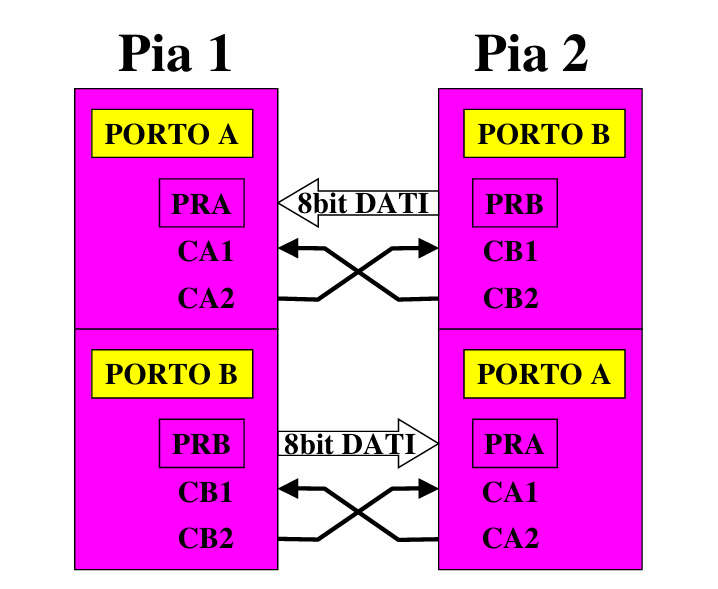
\includegraphics[width=0.75\textwidth]{img/PIA_fd.png}
    \caption{Configurazione Full Duplex}\label{img:PIA_FD}
\end{figure}

Le routine dedicate alla configurazione dei porti A e B sono uguali a quelle viste nell'esercizio 2 di questa sezione (\ref{par:es_1_2}).
La routine dedicata alla configurazione del terminale consta di una sola istruzione e ritorna:

\begin{lstlisting}
    DVTER	MOVE.B	#$3f,TERC	;seleziona indirizzo stato/controllo
	RTS		
\end{lstlisting}

In pratica viene soltanto scritto il bye 00111111 nel registro di controllo/stato del terminale, il cui significato è chiarito dall'immagine \ref{img:terminal_cfg}.

\begin{figure}[!ht]
    \centering
    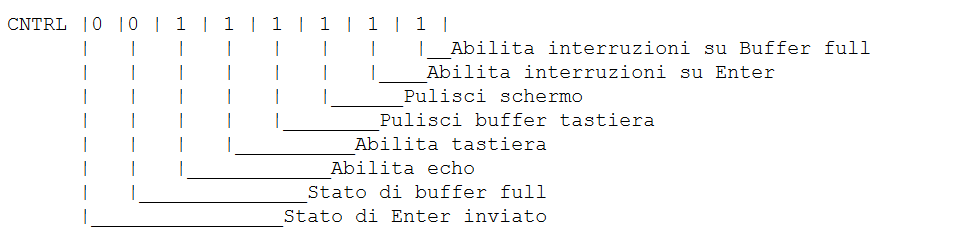
\includegraphics[width=0.5\textwidth]{img/terminal_ctrl.png}
    \caption{Configurazione registro controllo/stato del terminale}
    \label{img:terminal_cfg}
\end{figure}

Dopodichè, il main entra in un ciclo idle in cui attende le interruzioni (dopo averle abilitate sul registro di stato).
Vediamo nel dettaglio la ISR per la gestione dato proveniente dalla tastiera di TERMINAL e spedito, per tramite del PIA porto B, all'altro sistema.
ISR associata all'interrupt di liv. 1, \#vect 25 mappato a \$64 della ROM con ISR a \$8500. 

\begin{lstlisting}
    ORG	$8500		ricevi da tastiera
    INT1	MOVE.L	A0,-(A7)		;push di A0,A1,A2,D0,D1 in stack supervisor
        MOVE.L	A1,-(A7)
        MOVE.L	A2,-(A7)
        MOVE.L	D0,-(A7)
        MOVE.L	D1,-(A7)
        MOVEA.L	#TERD,A0
        MOVEA.L	#PIADB,A1
        MOVEA.L	#PIACB,A2
    
    INPUT	MOVE.B	(A0),D0			;acquisisci dato da terminal
    
    *trasferisci il carattere letto alla PIA-B con handshaking
            MOVE.B  (A1),D1         ;lettura fittizia 
            MOVE.B  D0,(A1)         ;Dato su bus di PIA porto B: dopo la scrittura di PRB, CB2 si abbassa
    *								;cio fa abbassare CA1 sulla porta gemella dell'altro sistema generando 
    *								;un'interruzione che coincide con il segnale DATA READY
        
    ciclo2	MOVE.B	(A2),D1			;In attesa di DATA ACKNOWLEDGE
        ANDI.B	#$80,D1				;aspetta che CRB7 divenga 1
        BEQ	ciclo2
                
    *fine trasferimento e handshaking
        
        CMP.B   	#13,D0		;Se il carattere ricevuto  ENTER	
        BNE     	INPUT		;termina altrimenti prossimo carattere
        ORI.B	#$1C,TERC		;riabilita tastiera ,pulisce buffer e video
        MOVE.L 	(A7)+,D1		;ripristino di D0,D1,A2,A1,A0
        MOVE.L	(A7)+,D0
        MOVE.L	(A7)+,A2
        MOVE.L	(A7)+,A1
        MOVE.L	(A7)+,A0
        RTE
\end{lstlisting}

In questo caso è presente per forza di cose un ciclo improduttivo (ciclo2) perchè bisogna procedere sequenzialmente al set di istruzioni successivo che prevede un salto a INPUT se il carattere ricevuto non è quello finale (ENTER). Dopodichè resetta il terminale riabilitando tastiera e pulendo buffer e video scrivendo nel registro di controllo in accordo a quanto esposto nella figura \ref{img:terminal_cfg}, e ritorna.

Procediamo vedendo la ISR per il \textit{buffer full}: praticamente è identica a quella per l'acquisizione del messaggio in seguito a ENTER, ma in questo caso vengono inviati tutti e 256 i caratteri conservati nel buffer del terminale.
ISR a \$8600 associata all'interrupt di livello 2 \#vect (24+2) => mappato a 4*26 = 104 = \$68.

\begin{lstlisting}
    ORG	$8600		
    INT2	MOVE.L	A0,-(A7)		;push di A0,A1,A2,D0,D1 in stack supervisore
        MOVE.L	A1,-(A7)
        MOVE.L	A2,-(A7)
        MOVE.L	D0,-(A7)
        MOVE.L	D1,-(A7)
        MOVE.L	D2,-(A7)
        MOVEA.L	#TERD,A0
        MOVEA.L	#PIADB,A1
        MOVEA.L	#PIACB,A2
        MOVE.B	#255,D2		;#caratteri da trasferire
        
    SWAP	MOVE.B	(A0),D0			;acquisisci dato da terminal
    
    *trasferisci il carattere letto alla PIA-B con handshaking
        MOVE.B  (A1),D1         ;lettura fittizia => serve per azzerare CRB7 dopo il primo carattere, altrimenti resta settato con l ack
        MOVE.B  D0,(A1)         ;Dato su bus di PIA porto B: dopo la scrittura di PRB, CB2 si abbassa
    *							;cio fa abbassare CA1 sulla porta gemella dell'altro sistema generando 
    *							;un'interruzione che coincide con il segnale DATA READY
        
        
    ciclo3	MOVE.B	(A2),D1		;In attesa di DATA ACKNOWLEDGE
        ANDI.B	#$80,D1		;aspetta che CRB7 divenga 1
        BEQ	ciclo3
                
    *fine trasferimento e handshaking
            
        DBRA    	D2,SWAP	;contatore di bit inviati	
        ORI.B	#$1C,TERC	;riabilita tastiera ,pulisce buffer e video
        MOVE.L	(A7)+,D2	;ripristino di D0,D1,A2,A1,A0
        MOVE.L 	(A7)+,D1
        MOVE.L	(A7)+,D0
        MOVE.L	(A7)+,A2
        MOVE.L  	(A7)+,A1
        MOVE.L  	(A7)+,A0
        RTE
\end{lstlisting}

L'ultima interruzione è quella che scatena il porto A in seguito alla ricezione di un carattere. 

\begin{lstlisting}
    ORG $8700		

    INT3    	ANDI.B		#%11101001,TERC	;disabilita: tastiera,cancella video,interruzioni su enter		 
        MOVE.L  A1,-(A7)		;salvataggio registri
        MOVE.L  A0,-(A7)
        MOVE.L  D0,-(A7)
    
        MOVEA.L  #TERD,A0	;inizializzazione indirizzi device
        MOVEA.L  #PIADA,A1
        
        MOVE.B 	(A1),(A0)	;acquisisce il carattere e lo trasferisce a Terminal
    *						;la lettura da PRA fa abbassare CRA7 e CA2 => nell'altro sistema si abbassa CB1
    *						;cio corrisponde all'attivazione di CRB7 che funge da DATA ACKNOWLEDGE
        
        MOVE.L  (A7)+,D0		;ripristino registri 
        MOVE.L  (A7)+,A0
        MOVE.L  (A7)+,A1
        
        ORI.B	#$12,TERC	;riabilita tastiera e interruzioni su enter 
        RTE
    
    
        END	BEGIN
\end{lstlisting}

\subsection{Considerazioni finali}
In conclusione, è utile chiarire che le linee di interruzione IRQA e IRQB sono direttamente collegate ai flag CRA7 e CRB7, che si alzano quando c'è una transizione attiva dei segnali CA1/CB1 rispettivamente.
I flag di interruzione CRA7/CRB7 vengono automaticamente abbassati dopo un'operazione di READ
sul porto corrispondente, e questo è il motivo per cui nella parte software è necessaria la \textit{lettura fittizia}. 
Per quanto riguarda i bit del registro di stato/controllo del dispositivo PIA, in questa esercitazione abbiamo visto la configurazione per il protocollo di comunicazione handshaking. Le altre modalità, definite in base ai bit 5,4 e 3 dei registri di controllo,disciplinano il momento in cui CA2/CB2 deve essere rialzato, quindi non cambia nulla
dal punto di vista delle funzionalità.